\lecture{12. I Will Forgive Their Iniquity}{12}

%------------------------------------------------------------------------------
\section{Introduction}

%--------------------------------------
\begin{frame}{God wants to have mercy on all}

\begin{center}

\includegraphics[height=0.8\textheight]{figures/ladyJustice.jpg}
\end{center}

\note{09:00}
\note[item]{This depiction of lady justice illustrates a few things we'd like to avoid when it comes to our spiritual life.}
\note[item]{The balance: What you've done will be weighed exactly against the standard.}
\note[item]{The blindfold: You can't get out of it because you're special.}
\note[item]{The sword: If the balance finds you guilty, consequences will follow.}
\note[item]{But, God arranged His plan specifically so He could show mercy}
\note[item]{It's hard for us to understand, because we're used to how our justice system works.}
\note[item]{Governments seek out the wrong-doers for the expressed purpose of bringing them to justice.}
\note[item]{Our Lord sought out wrong-doers to help them avoid the justice they deserve.}
\end{frame}



%--------------------------------------
\begin{frame}{God wants a relationship with people}
\framesubtitle{Jeremiah 31:31-34}
	\keyversehiglight{For I will forgive their iniquity, and I will remember their sin no more.}
\note{09:33}
\end{frame}

%--------------------------------------
\begin{goals}
\goal Know what sin is, why it separates us from God, and what God has done about it in the New Covenant
\goal Examine why it is easy for us to strive for perfect lawkeeping rather than faithfulness
\goal Consider ways to keep the guilt of past sins from damaging your current relationship with God

\note{09:35}
\end{goals}

%------------------------------------------------------------------------------
\section{Sin is everyone's problem}

%--------------------------------------
\begin{frame}{Law shows us what's right and wrong}
\framesubtitle{Romans 3:5-28}

\begin{itemize}
	\item Law brings a knowledge right and wrong
	\item We become aware of our sin.
	\item ``Men and brethren, what should we do?''
\end{itemize}

\note{09:38}
\end{frame}

%--------------------------------------
\begin{frame}{God's plan shows mercy to everyone}
\framesubtitle{Romans 3:5-28}

\begin{itemize}
	\item God is the judge
	\item He's also the only one who could provide a solution to sin.
	\item Thus, he is both just and justifier
	\item Under his New plan\ldots
	\begin{itemize}
		\item there is no room for boasting
		\item we live under a law of faith
		\item the law of works is satisfied
	\end{itemize}
\end{itemize}

\note{09:42}
\end{frame}

%--------------------------------------
\begin{frame}{Jesus is God's solution to sin.}
\framesubtitle{Hebrews 9:15-28}

\begin{itemize}
\item Jesus blood was a necessary condition for the New Covenant.
\item Jesus' death took care of sin once for all.
\item When he comes back he won't have to deal with sin again, but rather will deal with salvation.
\end{itemize}

\note{09:46}
\end{frame}

%------------------------------------------------------------------------------
\section{The importance of faithfulness}

\begin{frame}
\frametitle{`The Law' is both a thing and an idea}
\begin{center}
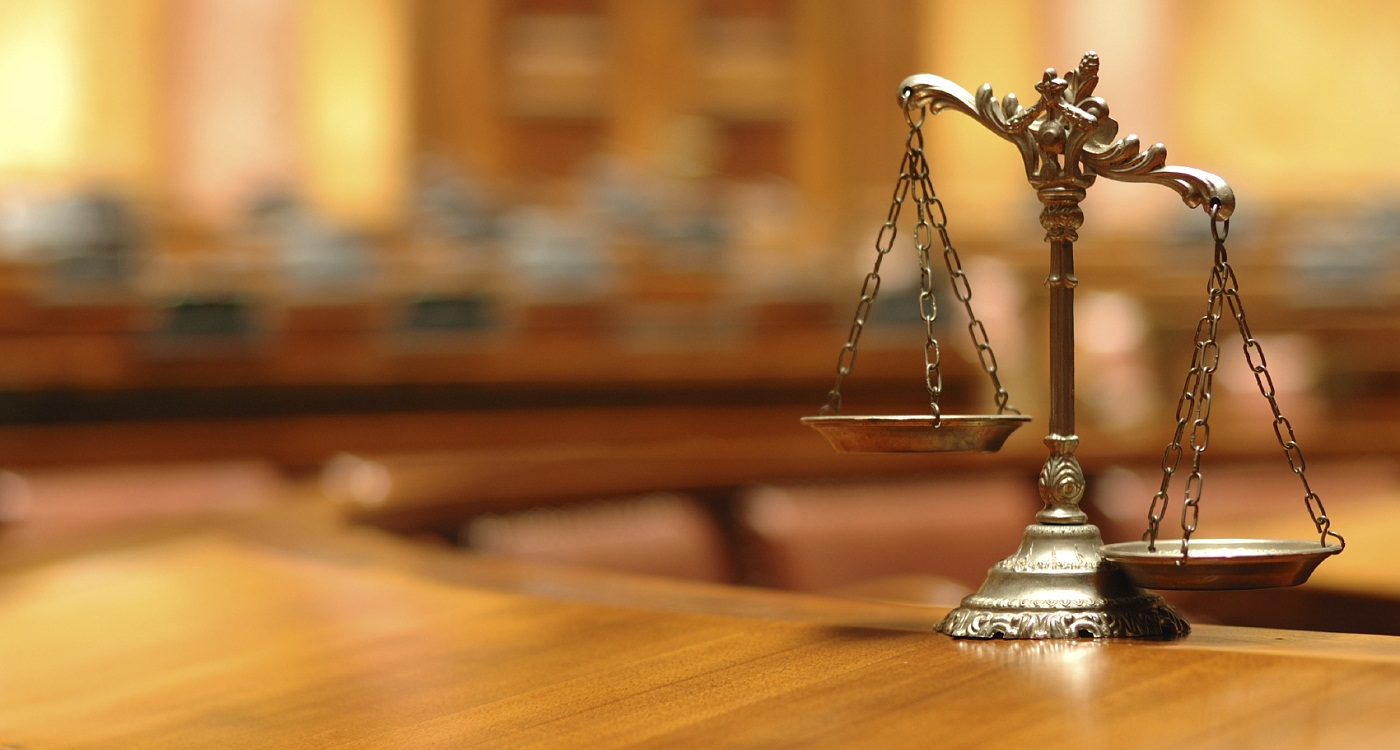
\includegraphics[width=0.8\textwidth]{figures/law.jpg}\\
The thing: The written Law of Moses\\
The idea: Justification through a system of works
\end{center}

\note{09:50}
\note[item]{We sometimes try to shoehorn every instance of the word `law' into meaning simply the Law of Moses.}
\note[item]{Why do we do that? Because there are many so-called `Christians' who would say that you don't have to do good works to go to heaven.}
\note[item]{These people misunderstand the word `law' to mean that \emph{any} attempt to do good works is futile and has no bearing on whether or not you enter heaven.}
\note[item]{So, to combat that, we say, `Well, these passages are talking about the Law of Moses, not just doing good works in general'.}
\note[item]{But, if we treat the word `law' as meaning simply the Law of Moses, we are taking large chunks of the New Testament and saying, ``That doesn't apply to me.''}
\note[item]{Paul in particularly uses the term `law' to fill a bigger concept.  And, it \emph{does}, I believe, have application for us.}
\end{frame}

%--------------------------------------
\begin{frame}{Life is hard for those who want to do right}
\framesubtitle{Romans 7:1-25}
\begin{itemize}
	\item There's always a conflict between the flesh and the spirit
	\item If you're in Christ, you'd like to \emph{never} sin.
	\item But, that doesn't happen.
	\item So, what do we do?
\end{itemize}
\note{09:55}
\end{frame}

%------------------------------------------------------------------------------
\section{Letting go of sin}

%--------------------------------------
\begin{frame}{There is no condemnation}
\framesubtitle{Romans 8:1-11}
\begin{itemize}
\item No condemnation exists for those in Christ
\item You are set free from sin
\item The requirements of the law are fulfilled in those who walk not in the flesh, but in the Spirit.
\end{itemize}

\note{10:00}
\end{frame}

%--------------------------------------
\begin{frame}{Faithfulness not perfection}
\framesubtitle{Hebrews 11:1}

\begin{itemize}
\item Faith \emph{is} our assurance.
\item Faith \emph{is} our conviction.
\item You have to trust God that he's forgiven your sins.
\item How do I get that faith? (Rom. 10:17)
\end{itemize}

\note{10:05}
\end{frame}

%------------------------------------------------------------------------------
\section{Review}

\begin{frame}{I Will Forgive Their Sins}
Sin separates us from God.
\begin{itemize}
	\item Law shows us what's right and wrong
	\item God's plan forgives our sins\ldots
	\item And, keeps Him just.
	\item The plan required the blood of Jesus
\end{itemize}
Our lack of perfection is frustrating
\begin{itemize}
	\item People who love God want to do what's right
	\item But we can be frustrated because we're not perfect.
	\item Jesus is the solution to those problems, too.
\end{itemize}
Have faith in your forgiveness
\begin{itemize}
	\item \emph{No} condemnation exists for those in Christ.
	\item You have to trust God.
	\item Bolster your faith through the Word.
\end{itemize}
	
\note{10:10}
\end{frame}
